\documentclass[10pt]{article}
\usepackage[hmargin={.5in},vmargin={.5in},foot={.6in}]{geometry}   
\geometry{letterpaper}              
\usepackage{color,graphicx}
\usepackage{setspace}
\usepackage{amsmath}
\usepackage{amssymb}
\usepackage{varioref}
\usepackage{textcomp}
\usepackage{textcomp}
\usepackage{mflogo}
\usepackage{wasysym}
\usepackage[normalem]{ulem}
\usepackage{hyperref}
\usepackage{booktabs}
\usepackage{natbib}

\newcommand{\HRule}{\rule{\linewidth}{0.25mm}}

\usepackage{fancyhdr} % This should be set AFTER setting up the page geometry
\pagestyle{plain} % options: empty , plain , fancy
\lhead{}\chead{}\rhead{}
\renewcommand{\headrulewidth}{.5pt}
\lfoot{}\cfoot{\thepage}\rfoot{}
\newcommand{\txtp}{\textipa}
\renewcommand{\rm}{\textrm}
\newcommand{\sem}[1]{\mbox{$[\![$#1$]\!]$}}
\newcommand{\lam}{$\lambda$}
\newcommand{\lan}{$\langle$}
\newcommand{\ran}{$\rangle$}
\newcommand{\type}[1]{\ensuremath{\left \langle #1 \right \rangle }}

\newcommand{\bex}{\begin{exe}}
\newcommand{\eex}{\end{exe}}
\newcommand{\bit}{\begin{itemize}}
\newcommand{\eit}{\end{itemize}}
\newcommand{\ben}{\begin{enumerate}}
\newcommand{\een}{\end{enumerate}}

\newcommand{\gcs}[1]{\textcolor{blue}{[gcs: #1]}}


\thispagestyle{plain}

\begin{document}

%\maketitle

\begin{center}
	\textbf{Adjective ordering in Tagalog: A cross-linguistic comparison}
\end{center}
Adjective ordering preferences determine the relative order of multi-adjective strings, for example, \emph{small black chair} vs.~\emph{black small box}, where the former is strongly preferred. Recently, \cite{scontrasetal2017adjectives} showed that adjective subjectivity is a robust predictor of ordering preferences in English: less subjective adjectives occur closer to the modified noun. The current study investigates the extent to which this pattern holds beyond English. We examine ordering preferences in Tagalog (Malayo-Polynesian: Western Malayo-Polynesian). Unlike English, Tagalog adjectives require a linking particle (\emph{-ng}/\emph{na}) in order to participate in modification structures \citep{foley1975,rubin1994}. Some authors analyze the semantic contribution of the linker similarly to that of conjunction \citep{rubin1994,scontrasnicolae2014}. In English, conjunction has been claimed to neutralize adjective ordering preferences \citep{fordolsen1975,byrne1979}. We therefore set out to determine (i) whether Tagalog possesses ordering preferences in the presence of linker, and, if so, (ii) to what extent subjectivity predicts those preferences.

\textbf{Expt.~1:} To determine the status of Tagalog ordering preferences, we replicated Expt.~1: \emph{Ordering preferences} from \citeauthor{scontrasetal2017adjectives} using Tagalog translations of the original English materials. 24 Tagalog-speaking participants indicated their preferences for pairs of multi-adjective strings formed from 26 unique adjectives from seven semantic classes, together with ten nouns; the pairs differed on the relative order of the adjectives (e.g., \emph{maliit na itim na silya} `small black chair' vs.~\emph{itim na maliit na silya} `black small chair'). On the basis of these naturalness ratings, we arrived at a single preferred distance measure for each adjective; values ranged from 0 (always preferred closest to the noun) to 1 (always preferred farthest from the noun). Fig.~1 plots these distance measures grouped by adjective class; there, we see that Tagalog does indeed have stable preferences, as evident in the significant deviation from chance (i.e., from 0.5) in nearly all of the distance measures.

\textbf{Expt.~2:} To determine the extent to which subjectivity predicts the Tagalog ordering preferences, we first measured adjective subjectivity in Tagalog using a faultless disagreement task (cf.~Expt.~1: \emph{Faultless disagreement validation} from \citeauthor{scontrasetal2017adjectives}). Eleven Tagalog-speaking participants indicated the extent to which two speakers could faultlessly disagree in the evaluation of an adjective property. For example, a trial might have speaker A state the Tagalog equivalent of `that chair is small.' Speaker B would counter with, `you're wrong, that chair is not small.' Participants judged whether both speakers could be right (coded as 1), or whether one must be wrong (coded as 0); to the extent that both can be right while disagreeing about a property, the property admits that degree of faultless disagreement, which measures adjective subjectivity. Averaging across participants, we calculated a single subjectivity score for each adjective. Fig.~2 plots adjective naturalness ratings against adjective subjectivity scores. In Tagalog, as in English, subjectivity is a reliable predictor of adjective ordering preferences (r$^2 = 0.54$, 95\% CI = $[0.22,0.74]$). Despite using diverging strategies to form modification structures, the two languages share the same adjective ordering preferences, which are predicted by adjective subjectivity.\\

\vfill

\noindent\begin{minipage}[t]{.56\textwidth}
	\begin{center}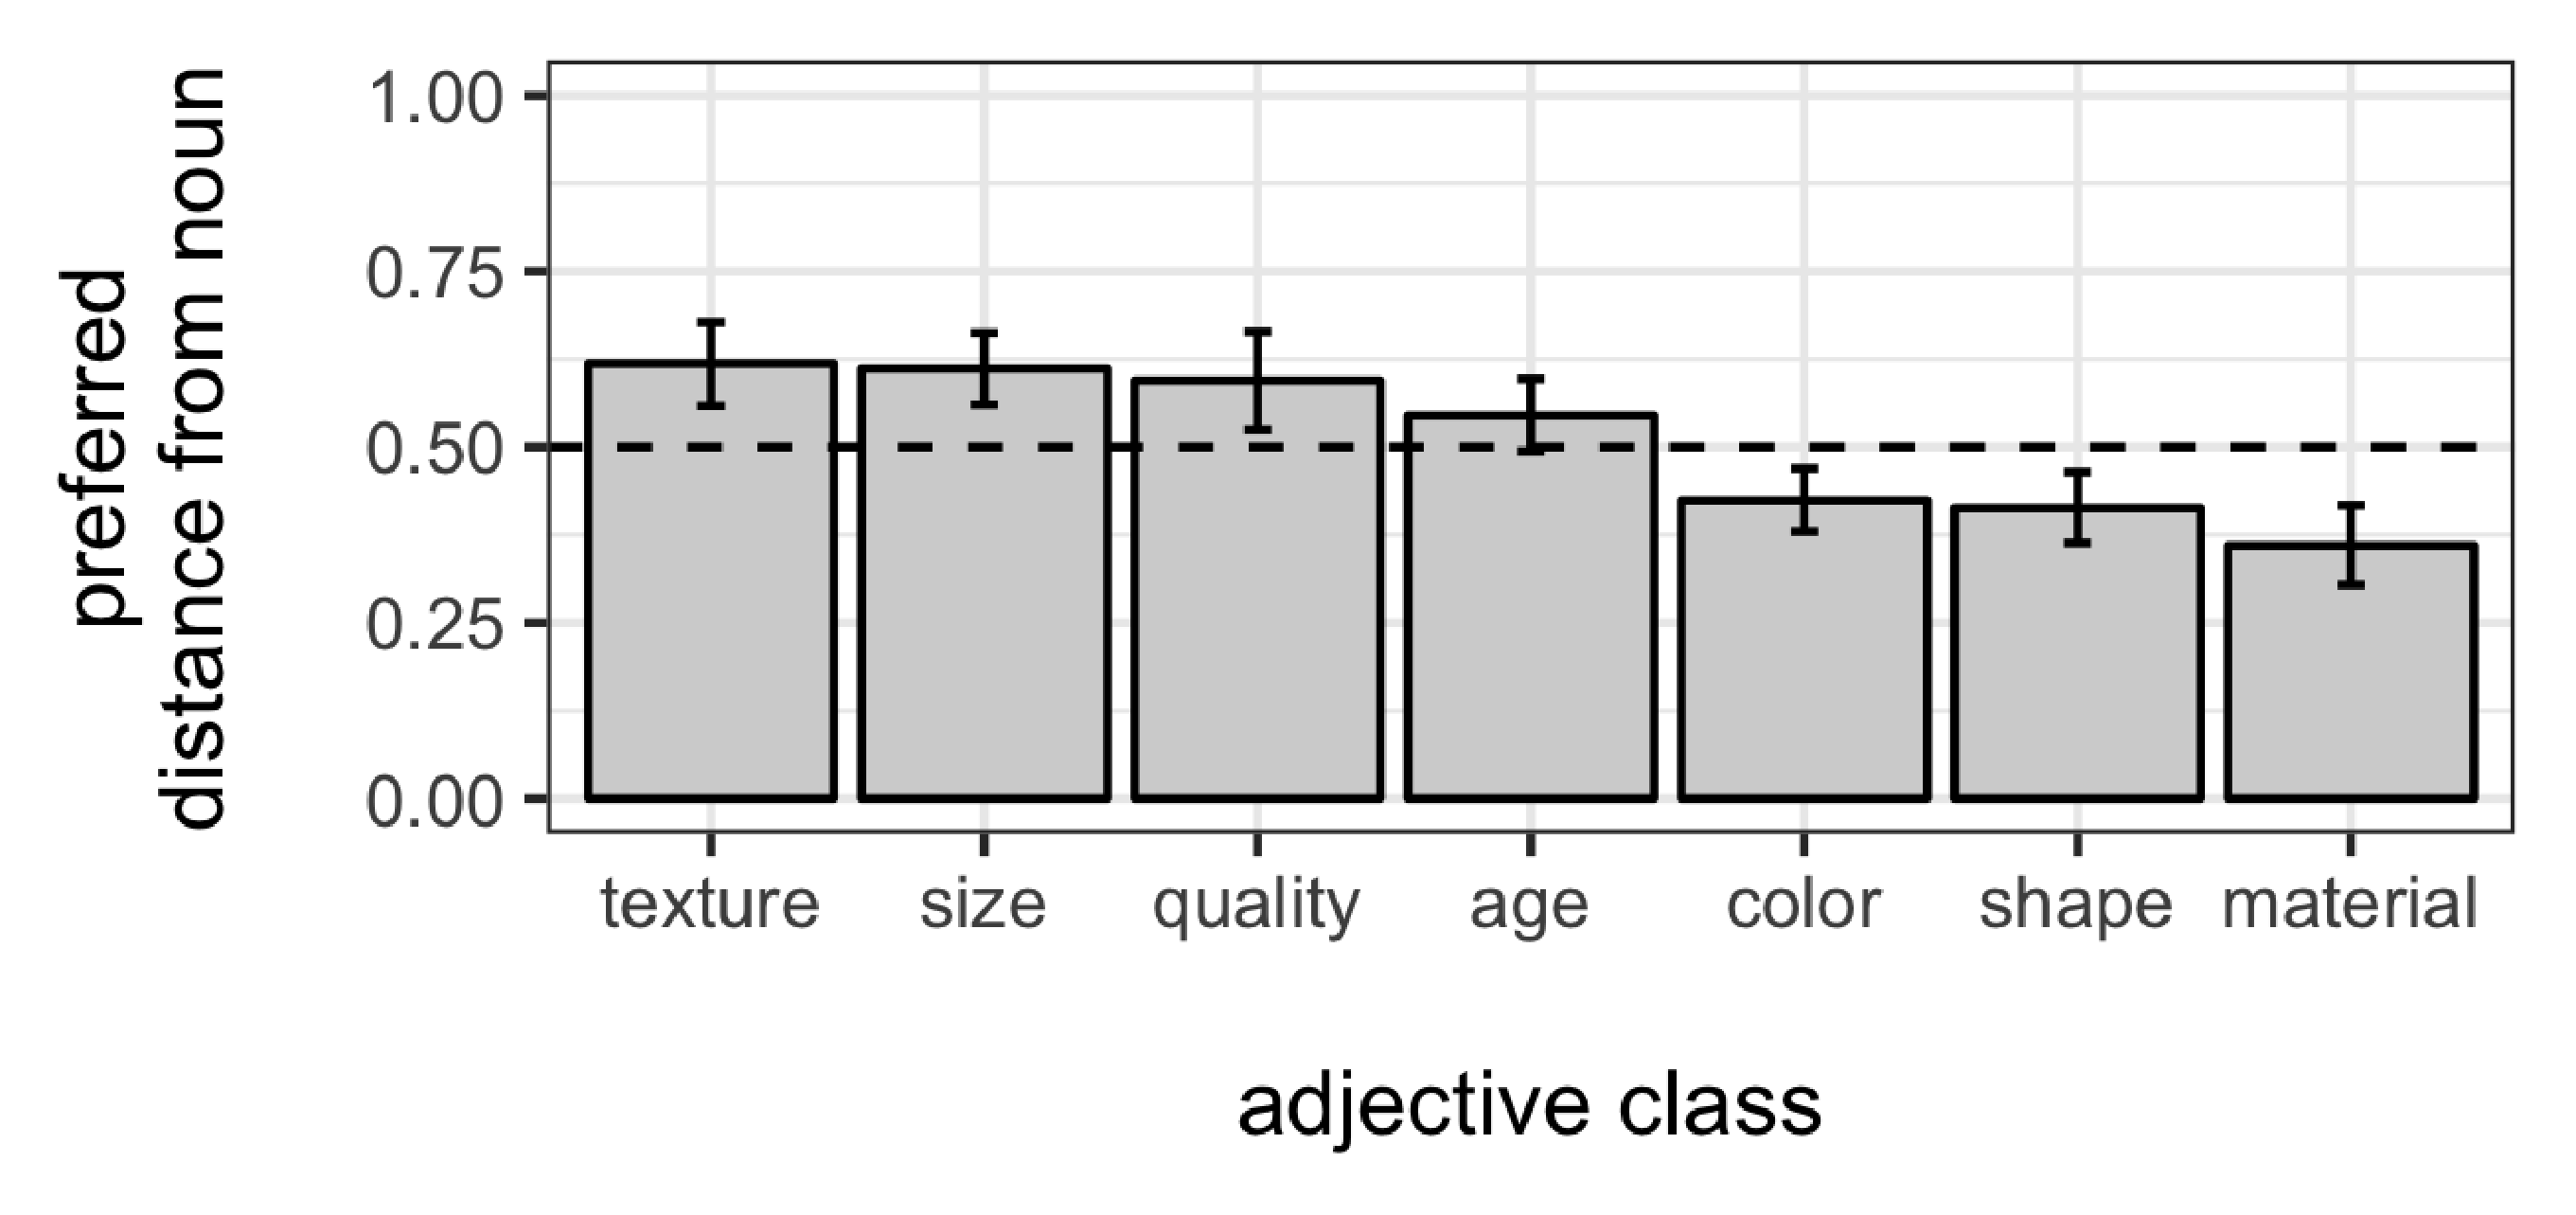
\includegraphics[height=1.8in]{../../experiments/2-tagalog-preference/results/LSA-class-distance.eps}
		\end{center}
	\vspace{-10pt}
	Fig.~1: Naturalness ratings from Expt.~1 grouped by adjective semantic class. Higher values indicate that a class's adjectives are preferred farther from the modified noun; lower values indicate that a class's adjectives are preferred closer. The dashed line indicates chance level, or the absence of stable preferences. Error bars represent bootstrapped 95\% confidence intervals drawn from 10,000 samples of the data.
	\end{minipage}
\hspace{10pt}
\begin{minipage}[t]{.4\textwidth}
	\begin{center}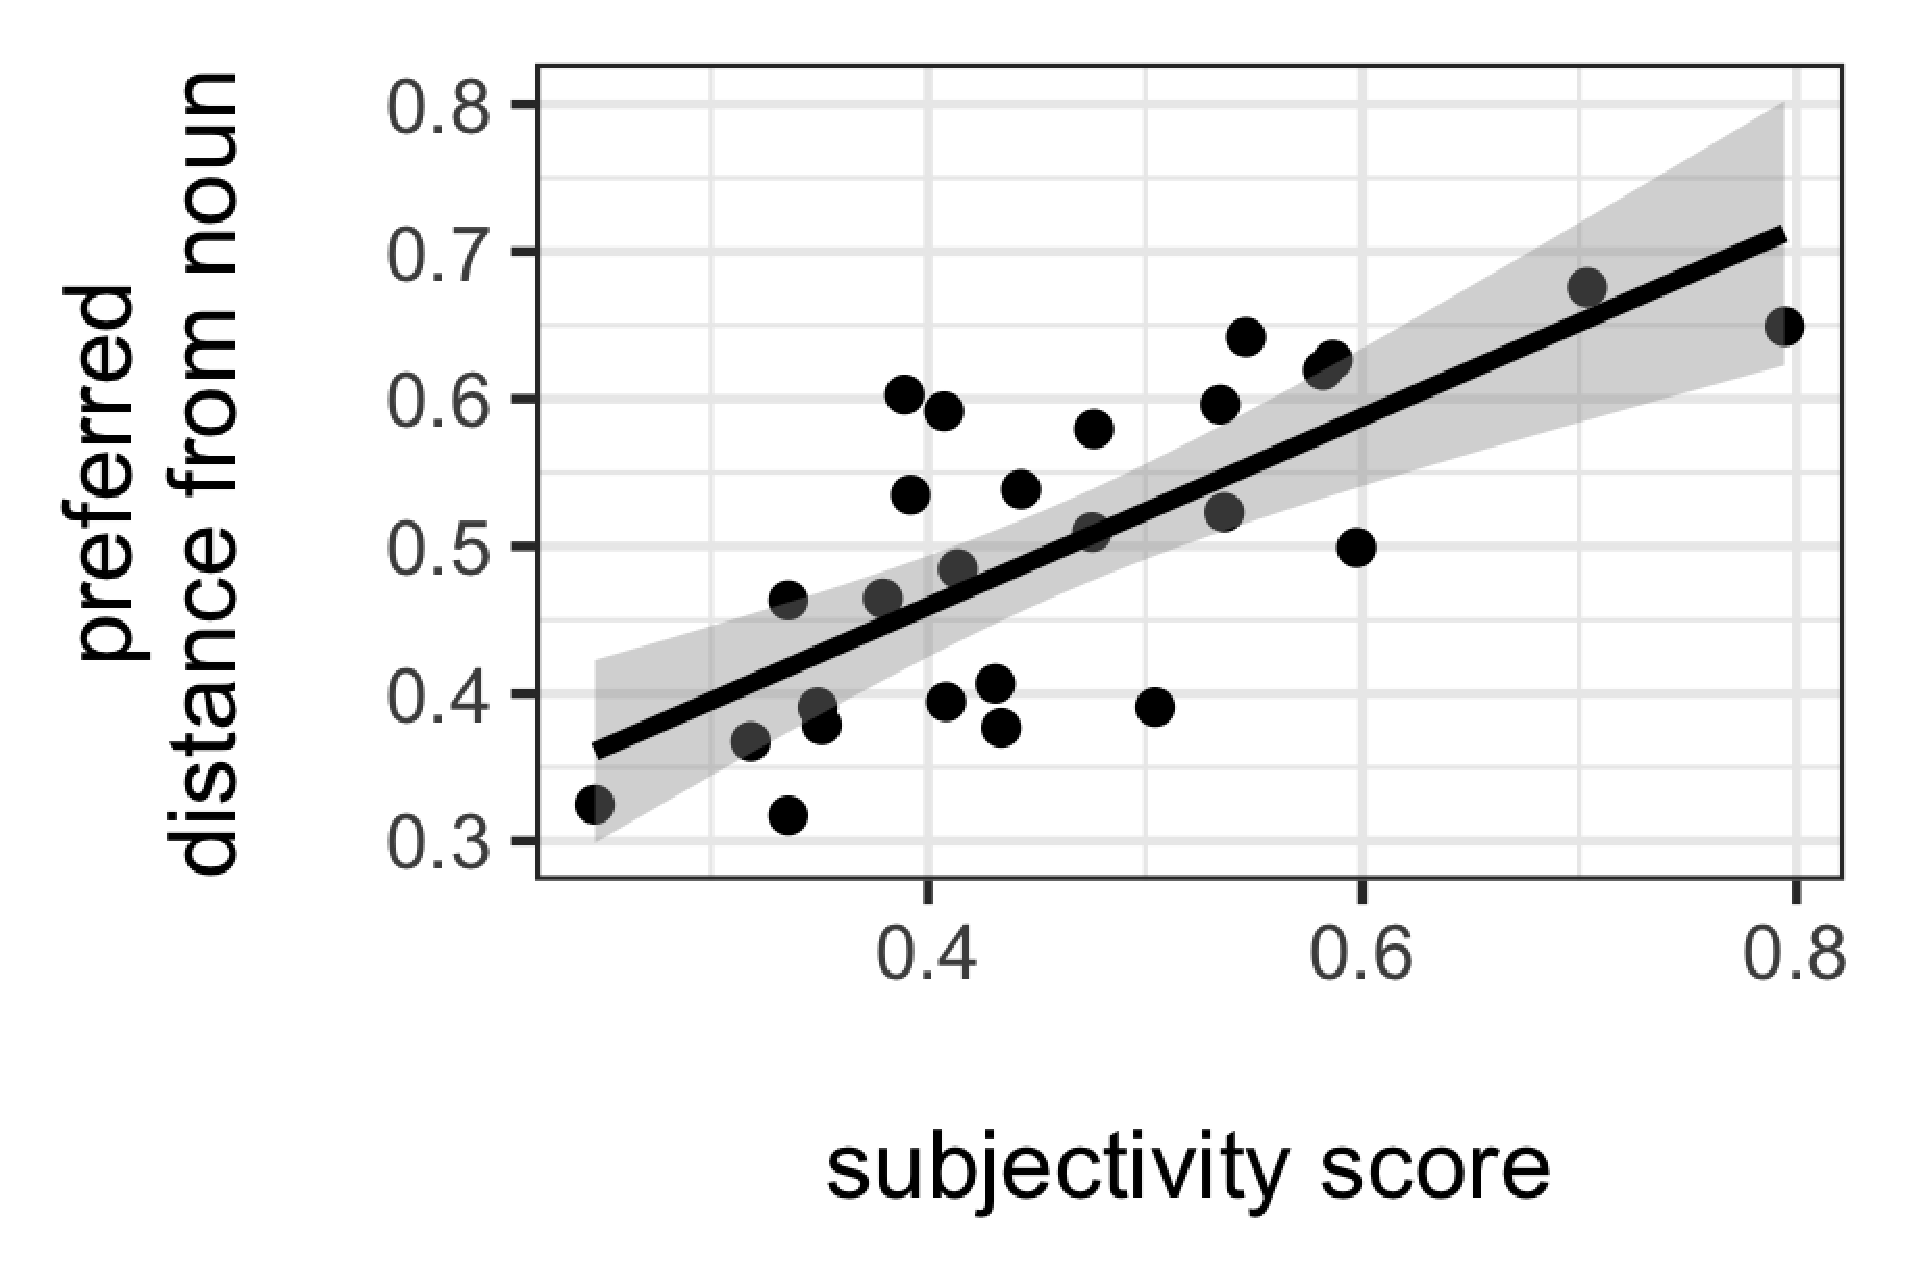
\includegraphics[height=1.8in]{../../experiments/2-tagalog-preference/results/LSA-naturalness-subjectivity.eps}
		\end{center}
	\vspace{-10pt}
	Fig.~2: Ordering preferences (obtained in Expt.~1) plotted against subjectivity scores (obtained in Expt.~2) for each of the 26 adjectives tested. Subjectivity accounts for 54\% of the variance in the ordering preferences (r$^2 = 0.54$, 95\% CI = $[0.22,0.74]$).
\end{minipage}

%From English to Hungarian to Mokilese, speakers exhibit strong ordering preferences in multi-adjective strings: ``the big blue box'' sounds far more natural than ``the blue big box.'' We show that an adjective's distance from the modified noun is predicted by the adjective's meaning: less subjective adjectives occur closer to the nouns they modify.  
%Subjectivity synthesizes---rather than supplants---many of the previous approaches to adjective ordering, incorporating notions like ``inherentness'' and ``context dependence'' into an intuitive psychological construct that readily operationalizes as a behavioral measure. 
%	We established two empirical constructs: first, the preferences themselves, which we measured using naturalness ratings (Expt.~1: 26 adjectives, n=45; Expt.~2: 70 adjectives, n=473) and validated with corpus statistics; and second, adjective subjectivity, which we measured directly (Expts.~3 \& 4; n=217) and corroborated with potential for faultless disagreement (Expt.~5: n=40). 
%An adjective's semantics predicts its distance from the modified noun, such that less subjective adjectives occur linearly closer to nouns they modify; subjectivity accounts for between 70\% and 85\% of the variation in our estimates of the ordering preferences (Fig.~1). %Word length and frequency also XXX. 
%To evaluate the \emph{relative} success of subjectivity, we investigated the predictions of three other hypotheses from the literature: intersective vs.~subsective modification (i.e., the mode by which an adjective composes semantically with the noun it modifies; \citealp{truswell2009}; Fig.~2), concept-formability (i.e., whether an adjective composes with a noun to form a complex, idiomatic concept; \citealp{McNally2004,bouchard2005,svenonius2008}; Fig.~3, top), and adjective inherentness (i.e., how essential an adjective's meaning is to the noun it modifies; \citealp{sweet1898,whorf1945}; Fig.~3, bottom). In each case, we found that subjectivity has greater predictive power. 
%\noindent 
%%While subjectivity accounts for the regularities we observe in adjective ordering, the deeper explanation for how subjectivity determines the relative order of adjectives remains unsettled. Our results suggest that ordering preferences likely emerge, at least partially, from a desire to place less subjective content closer to the substantive head of a nominal construction (i.e., closer to the modified noun). 
%%Subjective content allows for miscommunication to arise if speakers and listeners arrive at different judgments about a property description. Hence, less subjective content is more useful at communicating about the world. 
%%An explanation along these lines, based on pressures to facilitate successful reference resolution, would have to depend on the hierarchical, not linear, ordering of adjectives: noun phrases are built semantically outward from the noun, and more useful, less subjective content enters earlier in this process (cf.~the mirroring of preferences in pre- vs.~post-nominal languages). 
%%Whtever its source, 
%
%Adjective ordering preferences have received considerable attention throughout the history of generative grammar and cognitive psychology, owing to their remarkable stability within and across languages. %Something so robust, the reasoning goes, must evidence a deep principle of the cognitive architecture that shapes language. 
%Yet while descriptions of the phenomenon abound, an explanation continues to prove elusive. Our findings serve to narrow the space of possible explanations: rather than representing these preferences as a fully specified ranking according to semantic classes or syntactic projections, our results demonstrate that ordering preferences more likely emerge from a desire to place more informative, less subjective content closer to the substantive head of a nominal construction (i.e., closer to the modified noun). Subjective content allows for miscommunication to arise if speakers and listeners arrive at different judgments about a property description. Hence, less subjective content is more useful at communicating about the world. 
%An explanation along these lines, based on pressures to facilitate successful reference resolution, 
%would have to depend on the hierarchical, not linear, ordering of adjectives: noun phrases are built semantically outward from the noun, and more useful, less subjective content enters earlier into this process (cf.~the mirroring of preferences in pre- vs.~post-nominal languages). 
%The success of subjectivity in predicting adjective ordering preferences provides a compelling case where linguistic universals, the regularities we observe in adjective ordering, emerge from cognitive universals, the subjectivity of the properties that the adjectives name.\\

\vfill

%\newpage
{
  \bibliographystyle{chicago} 
  \renewcommand{\bibsection}{}
  \setlength{\bibsep}{0pt plus 0.3ex}
  \bibliography{greg}
}

\end{document}














